\documentclass[aspectration=1610,t]{beamer}
\usepackage{csc}
\title{Лекция 7. Тесты глубины и трафарета}


\date{
   \textbf{ИТМО}\\
   26 октября 2022\\
   Санкт-Петербург
}

\begin{document}

\begin{frame}
  \titlepage
\end{frame}

\begin{frame}[fragile]{Буфер глубины}
    Хранит определенную информацию для каждого фрагмента.
    \begin{itemize}
        \item Обычно, имеет размеры совпадающие с размерами буфера цвета.
        \item Буфер глубины для FBO по умолчанию создается оконной системой и хранит значения в виде 16, 24 или 32 битных числе.
        \item В большинстве систем по умолчанию создается буфер с точностью 24 бита.
    \end{itemize}
\end{frame}

\begin{frame}[fragile]{Буфер глубины}
    При включенном тесте глубины OpenGL
    {\small \begin{lstlisting}
glEnable(GL_DEPTH_TEST)
    \end{lstlisting}}
    \begin{itemize}
        \item производит проверку глубины каждого обрабатываемого фрагмента относительно данных, хранимых в буфере;
        \item при прохождении теста содержимое буфера будет обновлено значением глубины обрабатываемого фрагмента;
        \item при провале теста – хранимое значение останется прежним, а фрагмент отбрасывается.
    \end{itemize}
\end{frame}

\begin{frame}[fragile]{Ранний тест глубины}
    Тест глубины производится в экранном пространстве после выполнения фрагментного шейдера. В GLSL:
    \begin{itemize}
        \item {\bf gl\_FragCoord} в коде фрагментного шейдера хранит соответствующие координаты;
        \item {\bf (x, y)} - положение фрагмента;
        \item {\bf z} - значение для сравнения глубины.
    \end{itemize}
    В современных видеокартах используется трюк - {\bf ранний тест глубины}.
\end{frame}

\begin{frame}[fragile]{Настройка теста глубины}
    Очистка буфера для отрисовки очередного кадра:
    {\small \begin{lstlisting}
glClear(GL_COLOR_BUFFER_BIT | GL_DEPTH_BUFFER_BIT)
    \end{lstlisting}}
    Маска, позволяет производить сам тест, но не перезаписывать значение:
    {\small \begin{lstlisting}
glDepthMask(GL_FALSE)
    \end{lstlisting}}
    Функция, позволяет настроить поведения для сравнения:
    {\small \begin{lstlisting}
glDepthFunc(GL_LESS)
    \end{lstlisting}}
\end{frame}

\begin{frame}[fragile]{Функции для сравнения}
    \begin{figure}[htp]
        \centering
        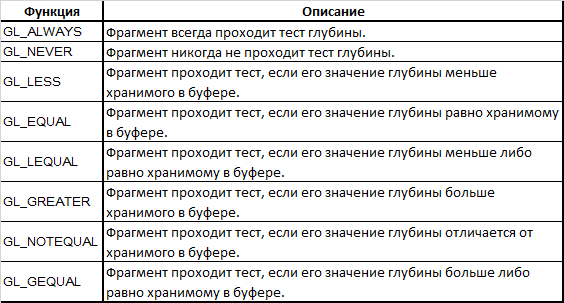
\includegraphics[scale=0.60]{res/depth_functions}
    \end{figure}
\end{frame}

\begin{frame}[fragile]{Z-Fight}
    Линейная интерполяция:
    $depth(z) = \frac{z - zNear}{zFar - zNear}$
    \begin{figure}[htp]
        \centering
        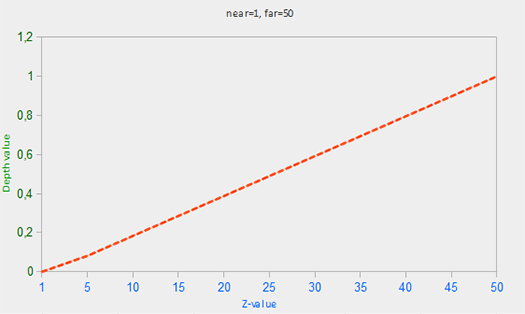
\includegraphics[scale=0.50]{res/lin_z}
    \end{figure}
\end{frame}

\begin{frame}[fragile]{Z-Fight}
    Для обратной величины:
    $depth(z) = \frac{z^{-1} - zNear^{-1}}{zFar^{-1} - zNear^{-1}}$
    \begin{figure}[htp]
        \centering
        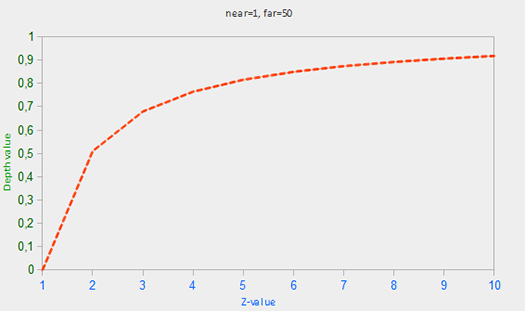
\includegraphics[scale=0.50]{res/frac_lin_z}
    \end{figure}
\end{frame}

\begin{frame}[fragile]{Z-Fight}
    Для преодоления проблем точности:
    \begin{itemize}
        \item не стоит располагать объекты слишком близко друг к другу (с риском наложения треугольников);
        \item задавать ближнюю плоскости отсечения как можно дальше;
        \item использовать формат буфера глубины с большей точностью.
    \end{itemize}
    В современных видеокартах используется трюк - {\bf ранний тест глубины}.
\end{frame}

\begin{frame}[fragile]{Визуализация буфера глубины}
    Простейший шейдер:
    {\small \begin{lstlisting}
void main() {             
    out_color = vec4(vec3(gl_FragCoord.z), 1.0);
}
    \end{lstlisting}}
    Для линеаризации значений, нужно обратить формулы.
\end{frame}

\end{document}

